% !TeX document-id = {1d88a3b2-9b5b-461b-9b0a-590d1c20474b}
% !TeX TXS-program:compile = txs:///pdflatex/[--shell-escape]
\documentclass[border={0 0mm 0 -1mm}]{standalone}
\usepackage{amsmath,amsfonts,amssymb}
\usepackage{tikz,pgfplots}
\usetikzlibrary{arrows,arrows.meta,bending,calc,decorations,shadings,shadows,shapes,shapes.arrows,shapes.geometric}
\usetikzlibrary{calc,fadings,decorations.pathreplacing}
\usepgfplotslibrary{units,fillbetween,groupplots,colorbrewer}
\usetikzlibrary{pgfplots.colorbrewer,}
\usepackage{pgfplotstable}
\usetikzlibrary{3d,spy}

\newcommand*{\xMin}{-2}%
\newcommand*{\xMax}{10}%
\newcommand*{\yMin}{-5}%
\newcommand*{\yMax}{7}%

\definecolor{As}{RGB}{255,255,0}
\definecolor{Al}{RGB}{173,216,230}
\definecolor{Ga}{RGB}{0,128,150}
\begin{document}
	
	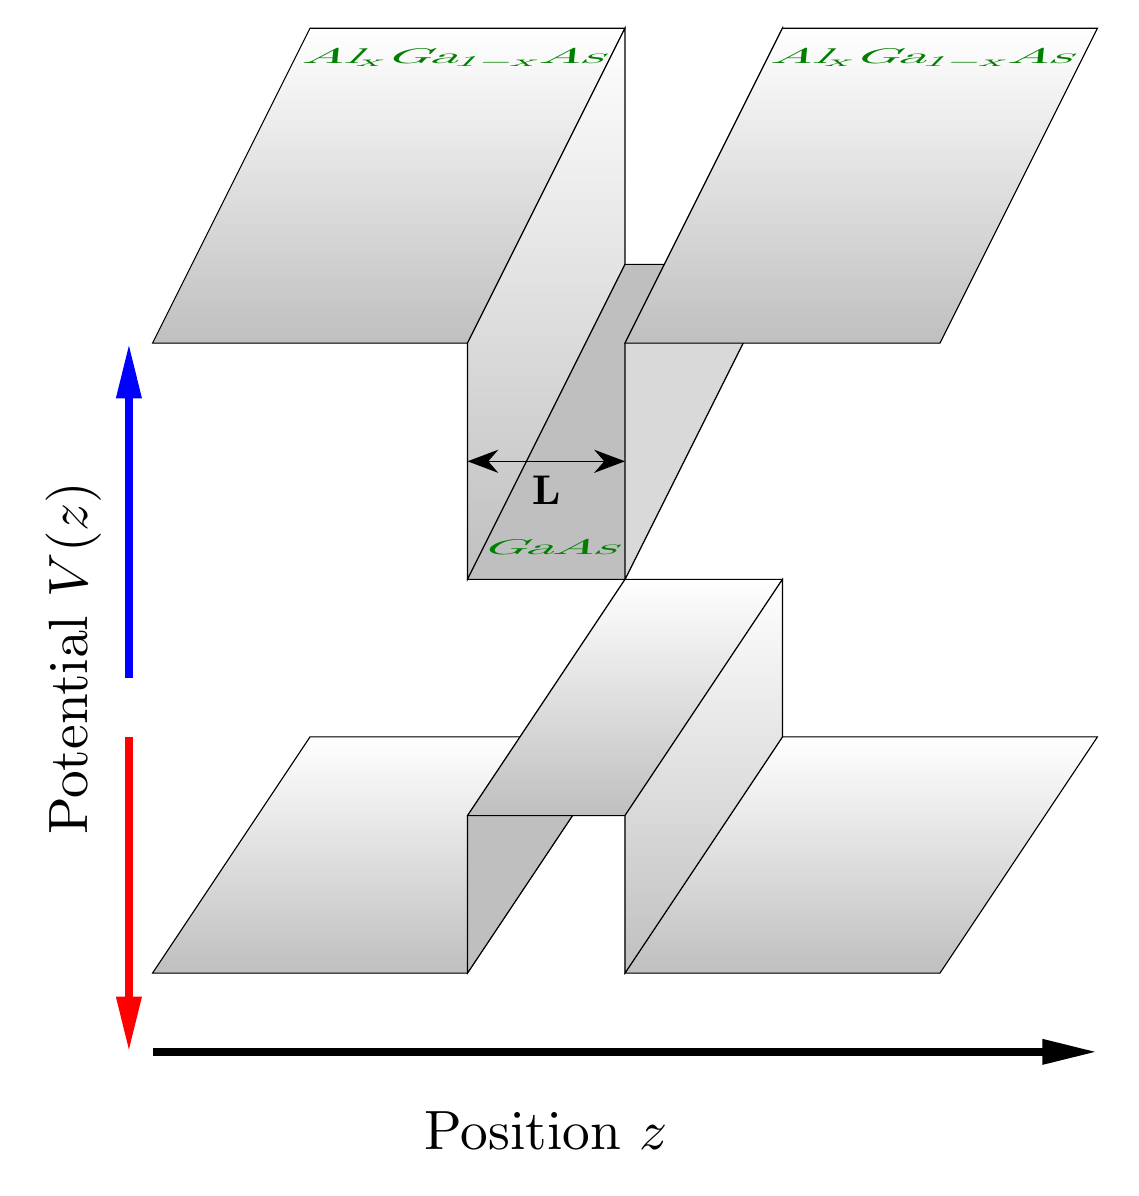
\begin{tikzpicture}
%		
%								\draw[step=.5cm,gray,very thin,opacity=0.2] (0,0) grid (\xMax,\yMax);
%								 \foreach \i in {\xMin,...,\xMax} {
%											\draw [very thin,gray,opacity=0.2] (\i,\yMin) -- (\i,\yMax)  node [below,opacity=1] at (\i,\yMin) {$\i$};
%										}
%								\foreach \i in {\yMin,...,\yMax} {
%											\draw [very thin,gray,opacity=0.2] (\xMin,\i) -- (\xMax,\i) node [left,opacity=1] at (\xMin,\i) {$\i$};
%										}
%		
		
%\filldraw[bottom color=gray!70!white, top color = white,decoration={random steps,segment length=1cm,amplitude=1mm}] (0,7)--(0,-2)--(4,-2)--(4,0)--(5,0)--
%(6,-2)--(10,-2)--(10,7)--(6,7)--(6,4)--(4,4);
%

%\filldraw[bottom color=gray!50!white, top color = white,decoration={random steps,segment length=1cm,amplitude=1mm},opacity=1] (-2,3)--(-2,-5)--(0,-2)--(0,7);
%
%
%
%\filldraw[bottom color=gray!50!white, top color = white,decoration={random steps,segment length=1cm,amplitude=1mm},opacity=0.5] (8,-5)--(8,3)--(10,7)--(10,-2);
%
%
%\filldraw[bottom color=gray!50!white, top color = white,decoration={random steps,segment length=1cm,amplitude=1mm},opacity=0.5,draw=none](-2,3)--(2,3)--(2,0)--(4,0)--(4,3)--(8,3)--(8,-5)--(4,-5)--(4,-3)--(2,-3)--(2,-5)--(-2,-5)--cycle;

\begin{scope}[rotate=0,xshift=3cm,yshift=1cm]	
\filldraw[bottom color=gray!50!white, top color = white] (-5,2)--(-1,2)--(1,6)--(-3,6)--cycle;
\filldraw[bottom color=gray!50!white,top color  = white](1,6)--(1,3)--(-1,-1)--(-1,2)--cycle;
\filldraw[gray!50!white,draw=black] (-1,-1)--(1,-1)--(3,3)--(1,3)--cycle;
\filldraw[gray!30!white,draw=black](1,2)--(1,-1)--(3,3)--(3,6)--cycle;
\filldraw[bottom color=gray!50!white, top color = white] (1,2)--(5,2)--(7,6)--(3,6)--cycle;

\draw[{Stealth[scale=2]}-{Stealth[scale=2]},line width=0.2mm] (-1,0.5)--node[below,font=\bf,scale=1.5] {L} (1,0.5);
\end{scope}


\begin{scope}[rotate=0,yshift=0cm,xshift=0cm]	
	\filldraw[bottom color=gray!50!white,top color=white] (0,-2)--(4,-2)--(2,-5)--(-2,-5)--cycle;
	\filldraw[bottom color=gray!50!white,top color=white] (6,-2)--(10,-2)--(8,-5)--(4,-5)--cycle;
	\filldraw[gray!50!white,draw=black] (2,-5)--(2,-3)--(4,0)--(4,-2)--cycle;
	\filldraw[bottom color=gray!50!white,top color=white] (2,-3)--(4,-3)--(6,0)--(4,0)--cycle;
	\filldraw[bottom color=gray!50!white,top color=white] (4,-5)--(6,-2)--(6,0)--(4,-3)--cycle;
	
\end{scope}
%\draw (4,1)--(6,1)--(8,6)--(6,6)--cycle;


\draw[-{Triangle[width=3mm,length=7mm]}, line width=1mm,blue](-2.3,-1.25) -- (-2.3, 3);
\draw[-{Triangle[width=3mm,length=7mm]}, line width=1mm,red](-2.3,-2.0) -- (-2.3, -6);
\draw[-{Triangle[width=3mm,length=7mm]}, line width=1mm,](-2.0,-6) -- (10, -6);
\node[rotate=90,scale=2] at (-3,-1) {Potential $V(z)$};
\node[rotate=0,scale=2,anchor=center] at (3,-7) {Position $z$};

\begin{scope}[canvas is zx plane at y=7,transform shape,every node/.style={scale=2}]
	\node [align=center,rotate=90,green!50!black] (Text) at (1,2.25) {$\mathrm{Al_{x}Ga_{1-x}As}$};	
	\node [align=center,rotate=90,green!50!black] (Text) at (1,8.2) {$\mathrm{Al_{x}Ga_{1-x}As}$};	
\end{scope}

\begin{scope}[canvas is zx plane at y=0.8,transform shape,every node/.style={scale=2}]
		\node [align=center,rotate=90,green!50!black] (Text) at (1,3.5) {$\mathrm{GaAs}$};	
\end{scope}
\end{tikzpicture}
	

\end{document}